%!TEX root = document.tex

%%%%%%%%%%%%%%%%%%%%%%%%%%%%%%%%%%%%%%%%%%%%%%%%%%%%%%%%%%%%%%
\begin{figure}[t!]
\centering
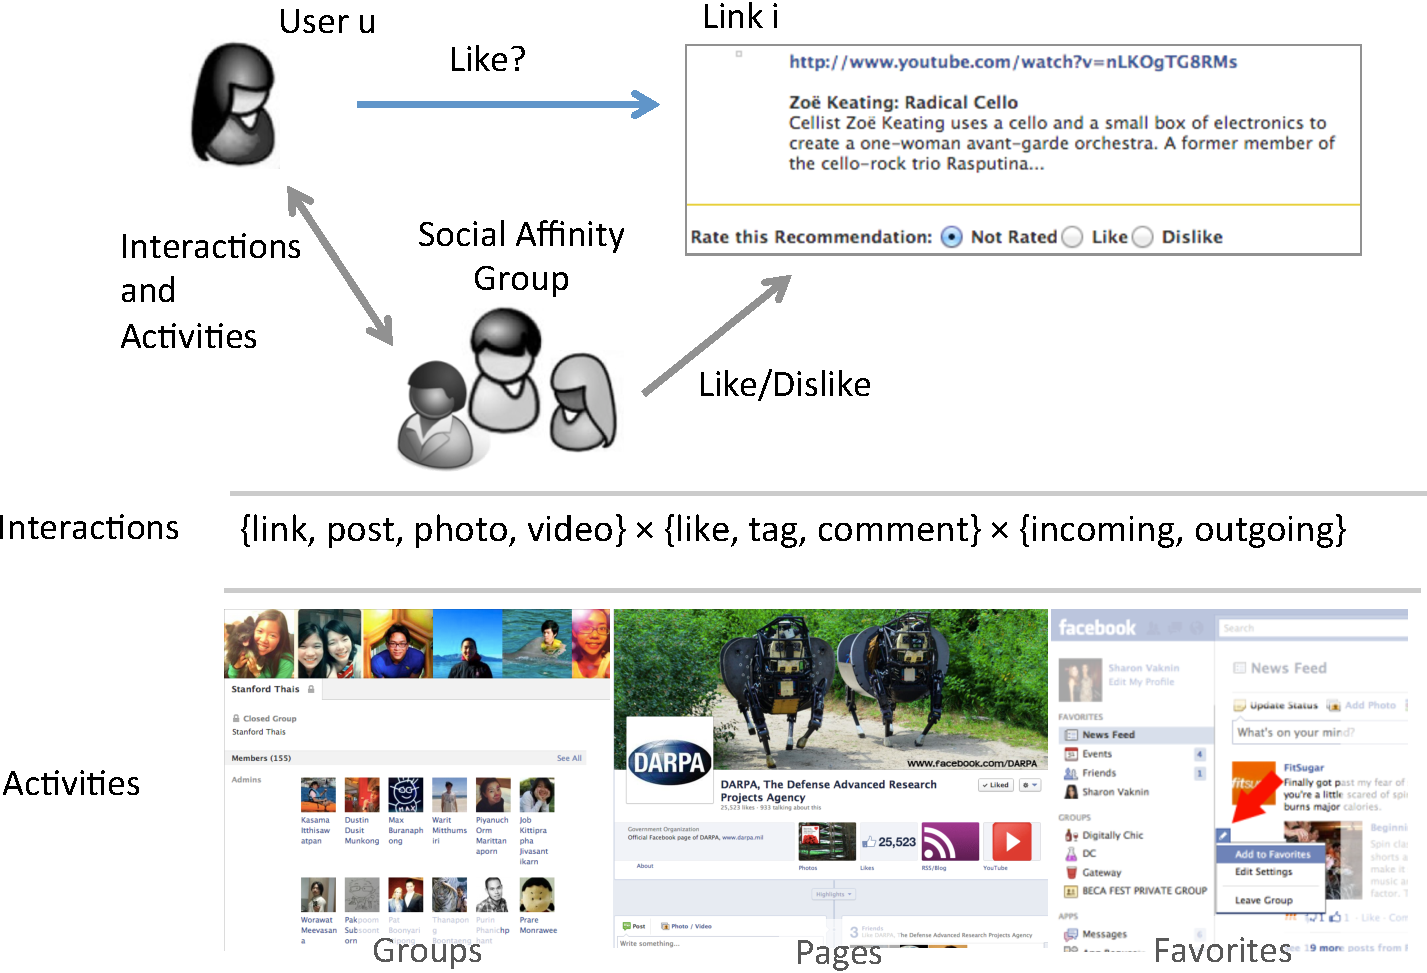
\includegraphics[width=1\linewidth]{data/overview}
\caption{Overview of social affinity for link recommendation.
A \emph{social affinity group (SAG)} consists of the set of alters 
of a user $u$ (ego) who have a
certain interaction or share an activity membership with $u$.
Alters defined by SAGs serve as proxies for an ego's interest with some
SAGs showing stronger affinity with an ego as learned by \emph{social affinity filtering (SAF)}
and analysed subsequently.}
\label{fig:overview}
\end{figure}
%%%%%%%%%%%%%%%%%%%%%%%%%%%%%%%%%%%%%%%%%%%%%%%%%%%%%%%%%%%%%%

As illustrated in Fig~\ref{fig:overview}, the high-level objective of
this work is to predict whether or not a user $u$ will like an item
$i$ (in our test case, a link posted on Facebook that may correspond
to a Youtube video, news or blog item, etc.).  Since the Facebook App
we have built for our experimental analysis collects explicit like and
dislike feedback, we define our prediction target of user $u$'s
preference for link $i$ as follows:
\begin{align*}
\likes(u,i) & \! := \! 
          \begin{cases}
	  \true    \!\! & \!\! \text{$u$ clicked \emph{like} for $i$}\\
	  \false   \!\! & \!\! \text{$u$ clicked \emph{dislike} for $i$}\\
          \unknown \!\! & \!\! \text{$u$'s preference for $i$ is unobserved}
	  \end{cases}
\end{align*}
From the observed data (i.e., instances of $\likes(u,i)$ evaluating to
$\true$ or $\false$)
%\footnote{$\likes(u,i)$ is not fully observed
%for all users $u$ and all links $i$.}, 
we learn to predict $\like(u,i)$ based on the surrogate link
preferences $\like(v,i)$ of sets of other Facebook users $v$ who have
at least one interaction or activity in common with $u$.  On Facebook,
there are many ways to define such sets of alters for the ego's
preferences as detailed in the next section.

\subsection{Interactions and Activities on Facebook}

On Facebook, we use the term {\em interactions} and {\em activities}
to refer to the range of user-user and user-community actions,
respectively.

{\bf Interactions} describes the communication between Facebook users. There are a few dozen different interaction types that have distinct item modality, action and direction defined
as follows:
\begin{itemize}
\item \textbf{Modality:} (4 possibilities)
User $u$ can interact with another user $v$ via \textit{links, posts, photos} and \textit{videos} that appear in either user's timeline.

\item \textbf{Action type:} (3 possibilities)
A user $u$ can \textit{comment} or \textit{like} 
user $v$'s item. He/she can also \textit{tag} user $v$ on an 
item, often indicating that user $v$ is present when the content is created (for photo/video/post), 
or to explicitly raise user $v$'s attention for a post --- with one exception in Facebook that $u$ cannot tag a link with users $v$ since the link is created by third parties and merely shared on Facebook.

\item \textbf{Directionality:} (2 possibilities)
We look at \textit{incoming} and \textit{outgoing} interactions, i.e.,
if user $u$ comments on, tags, or likes user $v$'s item,
then this is an outgoing interaction for $u$, and an incoming interaction for $v$.
Although high correlation between \textit{incoming} and \textit{outgoing} interactions 
has been observed~\cite{saez2011high}, whether interaction direction 
affects user preferences differently is still an open question we wish to answer
in this work. 
%then $u$ is in the set of incoming interactions for $v$
%and $v$ is in the set of outgoing interactions for $u$.
      								
\end{itemize}

There are a total of 22 interaction types. Namely the cross-product of modalities, actions and directions, minus {\em link-tag-\{incoming, outgoing\}} since links cannot be tagged in Facebook.

%\subsection{Activities}
%\noindent
% Can we insert more specific links to Facebook blog?  -SPS


{\bf Activities} describes the user interactions with Facebook
communities like groups, pages, and favourites defined as follows:
\begin{itemize}
  \item \textbf{Groups} on Facebook 
\footnote{From Facebook Blog: 
\surl{http://www.facebook.com/blog/blog.php?post=324706977130}, ``Groups are the place for small group communication and for people to share their common interests and express their opinion. Groups allow people to come together around a common cause, issue or activity to organise, express objectives, discuss issues, post photos and share related content.'' 
\label{fn:fbblog}}
are analogous to community organisations in the real-world. It allows
  users to declare membership and supports people to organise
  activities, to post related content, and to have recurring
  discussions about them.  Examples of groups include {\em Stanford
  Thai} (Fig~\ref{fig:overview} bottom left), or {\em Harvard Debate
  Club}.  \item \textbf{Pages} on Facebook \footnote{From Facebook
  Blog:
  (\surl{http://www.facebook.com/blog/blog.php?post=324706977130}
  ``Facebook Pages enable public figures, businesses, organisations
  and other entities to create an authentic and public presence on
  Facebook. Facebook Pages are visible to everyone on the Internet by
  default. Facebook users can connect with these Pages by becoming a
  fan and then receive their updates and interact with them.'' }
  %\footnotemark[\ref{fn:fbblog}] 
  are analogous to the homepages of people, organisations and events
  on the world-wide-web. They are publicly visible, and users can
  subscribe to the updates on the page, and also engage in
  discussions. Example pages include {\em DARPA} (an organisation,
  Fig~\ref{fig:overview} bottom middle), or {\em Beyonce} (a singer).

  \item \textbf{Favourites} are analogous to bookmarks (on physical
  books or on the web browser). It is a user-created list containing
  various items such as Facebook apps, books, music, and many other
  types of items to indicate their interest. Example favourite items
  include {\em Big Bang Theory} (TV series), or {\em FC Barcelona}
  (soccer club). Fig~\ref{fig:overview} bottom right shows a Facebook
  screenshot when a user adds a favourite.  \footnote{According to
  Facebook Blog, (\surl{https://www.facebook.com/help/232262810142682}
  ``Facebook facilitates a wide variety of user selected favourites
  (Activities, Favorite Athletes, Books, Interests, Movies, Music,
  Sports, Favorite Teams, Television). These favourites allow a user
  to associate themselves with other people who share their same
  favourite tendencies.''}
\end{itemize} 

Our evaluation includes 3000+ {\em group}, 4000+ {\em page} and
10000+ {\em favourite} features as detailed in
Sec~\ref{sec:datadesc}.

%% This is good text, but probably better in related work.  We have CIKM reviewers here who are
%% just skimming and trying to follow the technical setup in the initial sections... this
%% serves as a bit of a digression that detracts from some of the more important quantitative
%% points that we want to drive home with the reader as early as possible.  -SPS
\eat{
Note that the notion of affinity we adopt is based on direct user {\em
actions}, rather than static profile information, or structural
information of the social graph.  We believe this is a useful view
into the social network, as it was recently pointed out that a user's
attention (i.e., interactions) are divided among a small subset of
Facebook friends~\cite{backstrom2011center}, and that ratings of
real-world friendship strength seems to be more predictable from the
intimacy, intensity, and duration of interactions, than from social
distance and structural information~\cite{gilbert2009predicting}. Our
affinity definition is based on direct interactions within a users'
ego network, this is complementary to a recent
alternative~\cite{Panigrahy2012ubr} that uses number of paths between
two users to encode the resilience of network structure, as it was
recently found~\cite{Goel2012structure} that the vast majority of
information diffusion happens within one step from the source node. }
% interactions
%Our affinity
%\cite{Wilson2012BSG}


\subsection{Social Affinity Groups}
\label{ssec:sag}

\eat{
The major objective of this paper is to evaluate the effectiveness
of \textit{Social Affinity Filtering (SAF)} and fine grained analysis
of the informativeness of Interactions and Activities.We divide our
recommendation algorithm into two categories based on Interactions and
Activities of }

Based on the definitions of {\em interaction} and {\em activities}
above, we define two types of {\em social affinity groups (SAGs)} of a user $u$,
namely \textit{interaction social affinity groups
(ISAG)} and \textit{activity social affinity groups (ASAG)}.

\begin{itemize}
  \item \textbf{Interaction Social Affinity Groups (ISAGs)}: Let the set of
  interaction affinity classes be the cross-product of interaction
  modality, action, and direction:
  \begin{align*}
  	\textit{Interaction-Classes} := \, & \{\link, \post, \photo, \video\} \\
                                           & \times \{\like, \ttag, \comment\} \\
                                           & \times \{\incoming, \outgoing\}
  \end{align*}
  Then for $k \in \textit{Interaction-Classes}$ we define 
  \begin{align*}
     \textit{ISAG(u, k)} := \{ v | \textrm{user $v$ has had interaction $k$ with $u$} \}
  \end{align*}
  For example,
  \begin{itemize}
     \item \textit{ISAG(u, link-like-incoming)} is the set of all users who
     have liked a link posted \emph{by} user $u$, and 
     \item \textit{ISAG(u, photo-comment-outgoing)} is the set of all users whose photos
     user $u$ has commented \emph{on}.
  \end{itemize}
%% Mathematical definition
%% Do we need u for ASAGs?
\item \textbf{Activity Social Affinity Groups (ASAGs)}: We define activity affinity groups based on group membership, page likes and user favourites (of which there are over 17000 distinct activities in the set \textit{Activity-Groups} collected from our data).  For any one
of these activities $k \in \textit{Activity-Groups}$ we define:
  \begin{align*}
     \textit{ASAG(k)} := \{ v | \textrm{user $v$ has taken part in activity $k$} \}
  \end{align*}
%  \begin{quote} \textit{ASAG(u, k)} $:=$ the set of the users
%	who have common preference for entity $k$ (group, page,
%	favourite) with user $u$.  
%  \end{quote}
  For example,
  \begin{itemize}
     \item \textit{ASAG(page-Beyonce)} is the set of all users $v$ who 
     have liked \emph{Beyonce}'s Facebook \emph{page}, and 
     \item \textit{ASAG(group-Harvard Debate Club)} is the set of all users $v$ who 
     have joined the \emph{Harvard Debate Club}'s Facebook \emph{group}.
  \end{itemize}
\end{itemize}


\subsection{Social Affinity Features}

\label{ssec:SAfeature}

Given the previous definition of SAGs, we can now define two
sets of \emph{social affinity features} that can be used to train
classifiers for the purpose of social recommendation:

\begin{itemize} 
\item \textbf{Interaction Social Affinity Features (ISAFs)}: 
We define feature $X^{u,i}_k \in \{ \true, \false \}$ for user $u$, item $i$ and interaction
$k \in \textit{Interaction-Classes}$ as
  \begin{equation*}
   X^{u,i}_{k} \! := \!
      \begin{cases}
   		\true  \!\!\! & \exists v \in \mathit{ISAG}(u,k) \wedge \likes(v,i)\!=\!\true\\ 
   		\false \!\!\! & \text{otherwise}
      \end{cases}
  \end{equation*}
   In short, $X^{u,i}_{k}$ is $\true$ if any user sharing interaction $k$ with $u$ liked $i$.
   Here we note that $v$ is implicitly limited to $u$'s Facebook friends (with whom $u$
   may interact with).
%  Additionally we add friend feature which encodes whether the target 
%  item $i$ is liked by friend or not.
\item \textbf{Activity Social Affinity Features (ASAFs)}: 
We define feature $X^{u,i}_k \in \{ \true, \false \}$ for user $u$, item $i$ and activity
$k \in \textit{Activity-Groups}$ as
  \begin{equation*}
   X^{u,i}_{k} \! := \! 
      \begin{cases}
   		\true  \!\!\! & u \in \mathit{ASAG}(k) \wedge \\
                              & \exists v \in \mathit{ASAG}(k) \wedge \likes(v,i)\!=\!\true\\
   		\false \!\!\! & \text{otherwise}
      \end{cases}
  \end{equation*}
  In short, $X^{u,i}_{k}$ is $\true$ if both $u$ and some other $v$ are a member of activity $k$
  and $v$ has liked $i$.  Here we note that $v$ may range over all Facebook users (for which
  data has been collected), i.e., $v$ need not be a friend of $u$ to share the same activity $k$
  since activites are public.
\end{itemize}



\eat{
We train naive bayes, Logistic Regression(LR) and Support Vector
Machine(SVM) model with affinity features.  Logistic Regression and
SVM algorithm was implemented using \textit{LIBLINER} \cite{liblinear}
package.  We define Constant predictor as baseline predictor. Constant
predictor predicts the most common outcome in our datase ie disliket.
We compare the performance of Social Affinity Filtering with the state
of the art social collaborative filtering technique Social
MatchBox(SMB)\cite{SMB}.

In real world social networks activity features grows very quickly as number of user in social network increases. This motivates the fine grained
analysis of informativeness of social affinity features. Furthermore, fine grained analysis of interactions helps to understand the nature of user-user 
interactions and its predictiveness in greater detail. Hence, for the analysis of activities and interactions we rank the features using
\textit{Conditional Entropy}. 
\textit{Conditional Entropy} is defined as
\begin{quote}
\begin{math}
H(Y|X=\true) = \\-\sum_{y\in{(like,dislike)}} p(y|X$=$true)$ $log( p(y|X$=$true))
\end{math}
\end{quote}

With the data and methodology now defined including all dimensions of our analysis, we now proceed to an in-depth discussion of our findings.
}




 




